%%% Object Grasping Dataset 

\subsubsection{Object Grasping Dataset}
\label{sec:ObjectGraspingDataset}

In this section we present an object grasping dataset, collected at the University of Pisa, to be used within the PaCMan project.
Dataset contains a series of grasps performed on kitchen environment objects by a human operator using the Pisa/IIT SoftHand.
The goal of the dataset is to provide a grasp database for each object so that the relative pose between object and hand is always known during the grasp. This information can be later 
exploited to reproduce the grasp autonomously by a robot. 

The dataset is composed by sub-datasets, each one containing a single grasp recording performed on a kitchen environment object. The grasps are performed by a human operator, wearing
a motorized handle on his right arm, which supports and operates the Pisa/IIT SoftHand, the operator drives the SoftHand to grasp the object put on a table, while the system records all sensor data. 
\begin{figure}[tb!]
  \centering
  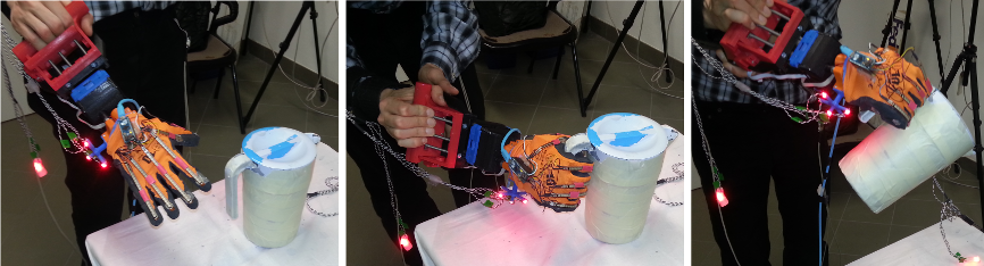
\includegraphics[width=0.955\textwidth]{GRP_subdb1.png}
  \caption{Pictures taken during the recording of the jug sub-dataset. The operator drives the SoftHand towards the object, then grasps and lifts it, while sensor data is being recorded.}
  \label{fig:grasp:subdb1}
\end{figure}
Figure~\ref{fig:grasp:subdb1} show photographs taken during the acquisition of a sub-dataset.
Each sub-dataset contains a single grasp type, the number of grasps associated with each object depends on its shape and grasp feasibility. A goal we kept in mind was to mimic human behaviour in grasping everyday objects,
for instance a cup was grasped by the handle, by the top without putting fingers inside it or by the sides and so on\ldots

Each grasp recorded is composed by a pre-grasp phase and an actual grasp phase. In the first, the operator moves the SoftHand towards the object and starts closing over the designated spot and in the latter the SoftHand 
closes on the object and lifts it up for a few seconds, then the object is put back on the table and the record stops. The user is able to distinguish between these two phases by reading sensor data: for instance joint positions
of each SoftHand finger is being recorded, so one can notice when the hand starts closing on the object or when it is just moving towards it.

The dataset is then populated by 8-10 seconds long records, each classified in sub-datasets according to the object name and grasp type. On each record the user has constant access to relative and/or absolute hand posture, object pose,
hand joints positions and point clouds of the whole scene. In fact the philosophy of the dataset was to collect as much data as possible during the grasp and then give the user the flexibility to chose which data to use for his application.
The remainder of the section describes which hardware was used during records and how it was configured, which software was used and finally a description and usage of data.

\paragraph{(a) Hardware setup used during dataset recording:}
%description of various hardware used
The whole system used to capture grasp recordings is composed by the following subsystems:
\begin{itemize}
  \item PhaseSpace Impulse Motion Tracking System.
  \item Pisa/IIT SoftHand.
  \item Handle for SoftHand.
  \item Flexi Force glove for SoftHand.
  \item Asus Xtion Pro Live.
\end{itemize}

The PhaseSpace Impulse system captures real-time motion by using cameras and LEDs.
The cameras detect the positions of the LEDs, which can be identified via an ID, and transmit the position of each LED in real-time at a frequency of 480Hz.
The main use of this system is to track the position of the SoftHand and the object to be grasped, so that the user has access to these data. 

To accomplish this feature two star-like prints were created to hold five LEDs each, one star was fixed to the SoftHand, the other on the object to be grasped.
Once calibrated the system identifies the two stars and attach a local reference system to them, which they give, respectively, the pose of the SoftHand and the object in space. %maybe explain better
In Figure~\ref{fig:grasp:star} pictures of the stars attached to the object and the SoftHand are visible.
\begin{figure}[bt!]
  \centering
  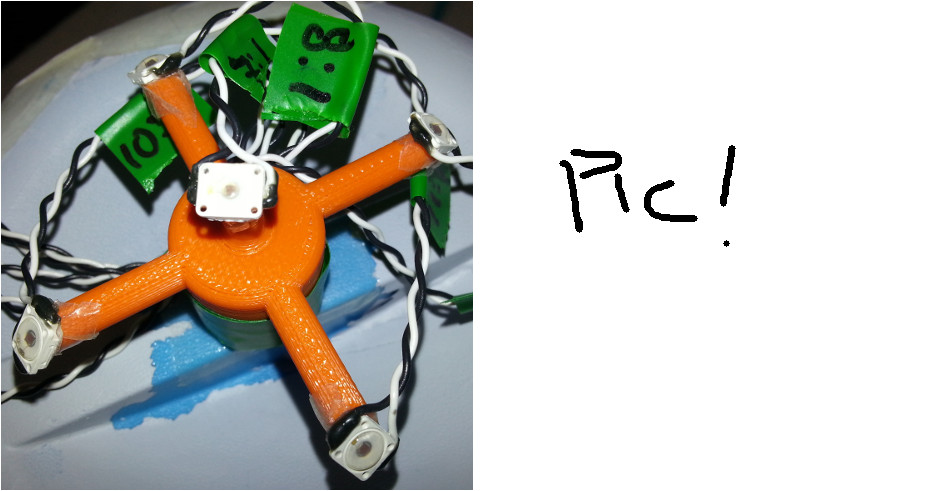
\includegraphics[width=0.95\textwidth]{GRP_star}
  \caption{The star with five LEDs used to track the pose of objects (left). The star used to track the SoftHand (right). The five unique LED IDs and their relative position, identify a local reference system for each star, which are then tracked by the PhaseSpace system.}
  \label{fig:grasp:star}
\end{figure}

The Pisa/IIT SoftHand was dressed with a special glove, called Flexi Force Glove, also designed at the University of Pisa.
Glove readings give a measure of finger bending and consequently joint angle values are estimated to be one third of the finger bending. This is a good approximation considering 
the SoftHand synergies and the type of application. Figure~\ref{fig:grasp:hand_glove} shows the SoftHand with and without the glove.
\begin{figure}[tb!]
  \centering
  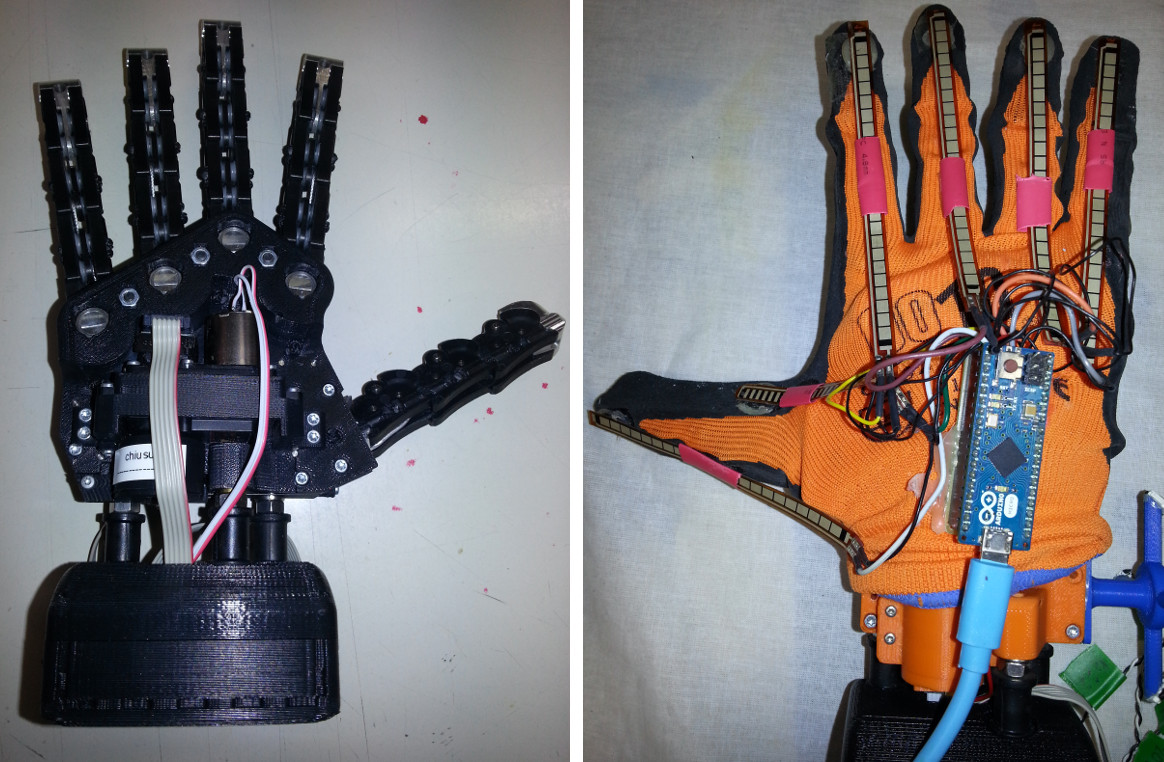
\includegraphics[width=0.95\textwidth]{GRP_hand_glove}
  \caption{The Pisa/IIT SoftHand without the FlexiForce Glove (left) and another one with it (right). Note the sensors alongside the hand fingers that measure the angular displacements.}
  \label{fig:grasp:hand_glove}
\end{figure}

Additionally, to ease the operator in manoeuvring the SoftHand a special support handle was created and used. This device can be attached to the operator's arm so that he can efficiently move and operate the SoftHand, similarly as he would with his own hand.
The handle has a lever to open and close the SoftHand with ease, a photograph of this device is visible in Figure~\ref{fig:grasp:handle}.
\begin{figure}[bt]
  \centering
  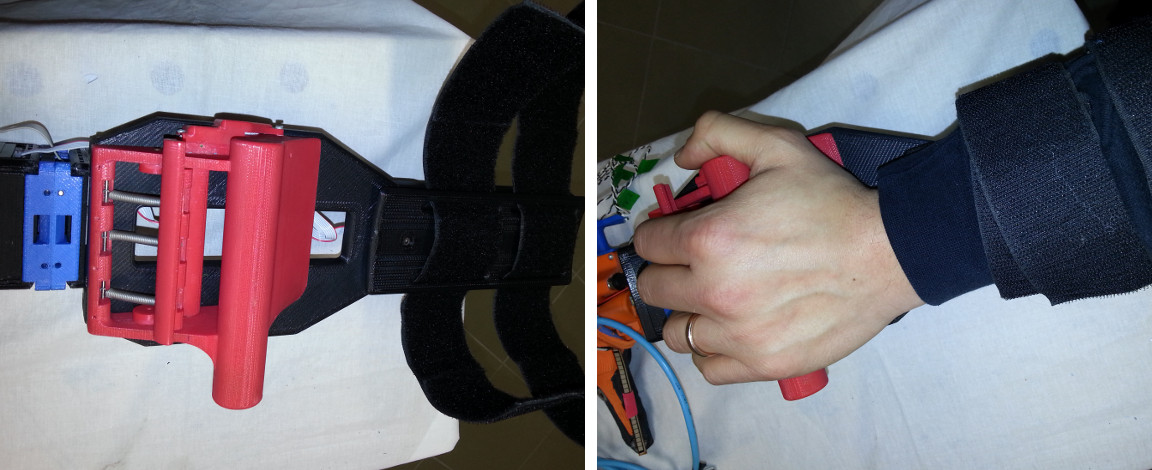
\includegraphics[width=0.95\textwidth]{GRP_handle}
  \caption{The handle for SoftHand without (left) and with (right) the operator's arm. The lever to close the SoftHand is located where the operator's hand should rest.}
  \label{fig:grasp:handle}
\end{figure}

Finally the Asus Xtion Pro Live RGB-D sensor was used to record point clouds and images of the scene while the grasp was recorded. This not only provides the user with more visual feedback, but it also gives more data that
could be post processed to analyze the grasp in a perceptual sense.
\paragraph{(b) Software setup used during dataset recording:}
%1mention we used ROS to sync various hardware
%2talk about calibration steps, and pose estimation paper
%3link and mention github repository where the software is stored
The software employed was developed under the Robot Operating System (ROS)~\cite{ROS} framework. ROS is an open-source set of software and tools widely used in robotics community,
that provides structured communications between heterogeneous hardware designed for robotics application in general.

For our scenario we needed a common platform to communicate with all the various hardware we used, so that recorded data is meaningful.
The software is available at the project website~\cite{website:pacman:dataset}, along with a description of the various packages used, the operative procedure to execute the grasps
and to play them back in any system without the need of the hardware we used. 
As a brief summary the software employs a communication framework like in Figure.~\ref{fig:grasp:software}, 
\begin{figure}[bt!]
  \centering
  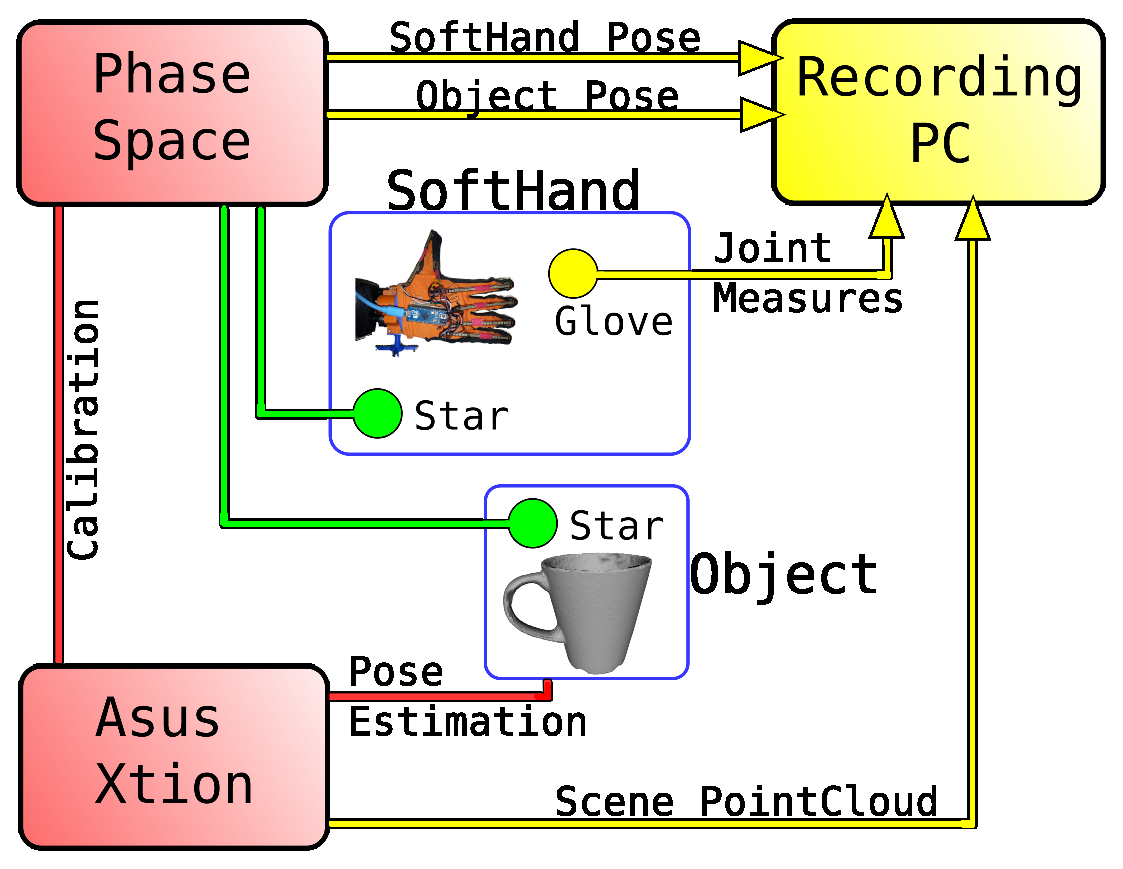
\includegraphics[width=0.95\textwidth]{GRP_scenario}
  \caption{Software infrastructure during grasp recording. Green connections represent PhaseSpace tracking of the two stars, red ones the calibration steps needed in order to communicate with different systems. Finally yellow connections represent recorded data during the grasp.}
  \label{fig:grasp:software}
\end{figure}
where all devices are configured and calibrated together. In order to provide meaningful data, the various systems need to be calibrated between each other, in particular: 
\begin{enumerate}
  \item First star and SoftHand, so that PhaseSpace can track SoftHand pose.
  \item PhaseSpace and Asus Xtion, to provide PointClouds and images consistent with the PhaseSpace.
  \item Second star and the object to be grasped, so that PhaseSpace can track the object pose.
\end{enumerate}

Calibration one was performed by knowing the SoftHand and star cad models and where the latter was fixed on the hand. So with concatenations of static geometric transformations, the two systems were calibrated with each other.
Since the transformation obtained is static and the star was never removed from the hand, the first calibration was performed just once and was not reported in Figure.~\ref{fig:grasp:software} for simplicity.

Second calibration is to be performed every time the system is rebooted and typically was performed once before the start of a recording session. 
This calibration procedure is available and detailed on the project website~\cite{website:pacman:dataset} under the calibration section of grasp dataset, so here, it is explained briefly.
The idea is to let the two systems track the same object, that we called the calibrator, so that they both produce the same output. If both tracking are precise the transformation between the two systems can be calculated
from concatenations of known transformations.

The last calibration is more involving, since it has to be performed every time an object is selected for grasping or an old one is replaced. This is performed by knowing the pose of the second star with respect to the PhaseSpace and the
pose of the object with respect to the Asus camera, now since the two systems are calibrated with each other (from previous calibration), the pose of the object with respect to the star is obtained by concatenating known transformations.
The calibration remains valid until the object is replaced or the star is moved from its fixed position.
Thus to obtain the last calibration we needed a procedure to obtain the object pose estimation with respect to the camera. To this end we developed a procedure to achieve online pose estimation of various objects with the Asus Xtion sensor
and the Point Cloud Library (PCL)~\cite{web:pcl}, the procedure is summarized here.

\begin{figure}[tb!]
  \centering
  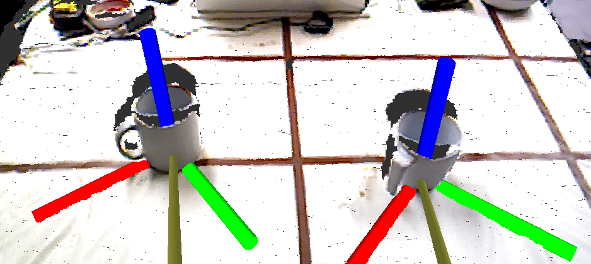
\includegraphics[width=0.95\textwidth]{GRP_poseestimation}
  \caption{A successful test result for the pose estimation procedure. Here two cups are correctly recognized from a scene and a local reference system is attached at their bottom, giving the pose estimation of the two objects with respect to the camera.
  The local reference system is built with z-axis (blue) aligned with the object vertical axis and x-axis (red) aligned with the cup handle.}
  \label{fig:grasp:pe}
\end{figure}

We employed four global 3D descriptors to obtain multiple representations of the same object geometry and combined these descriptors together with the aim of improving the performance and robustness of object recognition and pose estimation.
Then given an unknown object and database of known poses, for each descriptor, we first generated a list of ``k'' nearest neighbors. Then, we combined these lists for generating a composite list, which contains the neighbors agreed
by the majority of the descriptors. Finally, we extracted the best neighbor from this list by using an iterative refinement procedure that uses Iterative Closest Point (ICP) algorithm. The procedure was tested with real data acquired
with the Asus Xtion Pro sensor, results were satisfying so the procedure was successfully applied to our grasp dataset software. A result from the pose estimation procedure testing is visible in figure.~\ref{fig:grasp:pe}, the interested reader 
can find more details on the pose estimation procedure on this master thesis~\cite{thesis:spinelli}. 
%brief description of the procedure
\paragraph{(c) Data description and usage:}
Grasp recordings that populate each sub-dataset contain all the information gathered by all packages involved, in a single file. This special file, called bag file in ROS terminology, is an archive of all messages published
%explain exactly what is recorded and bagfiles
\begin{figure}[tb!]
  \centering
  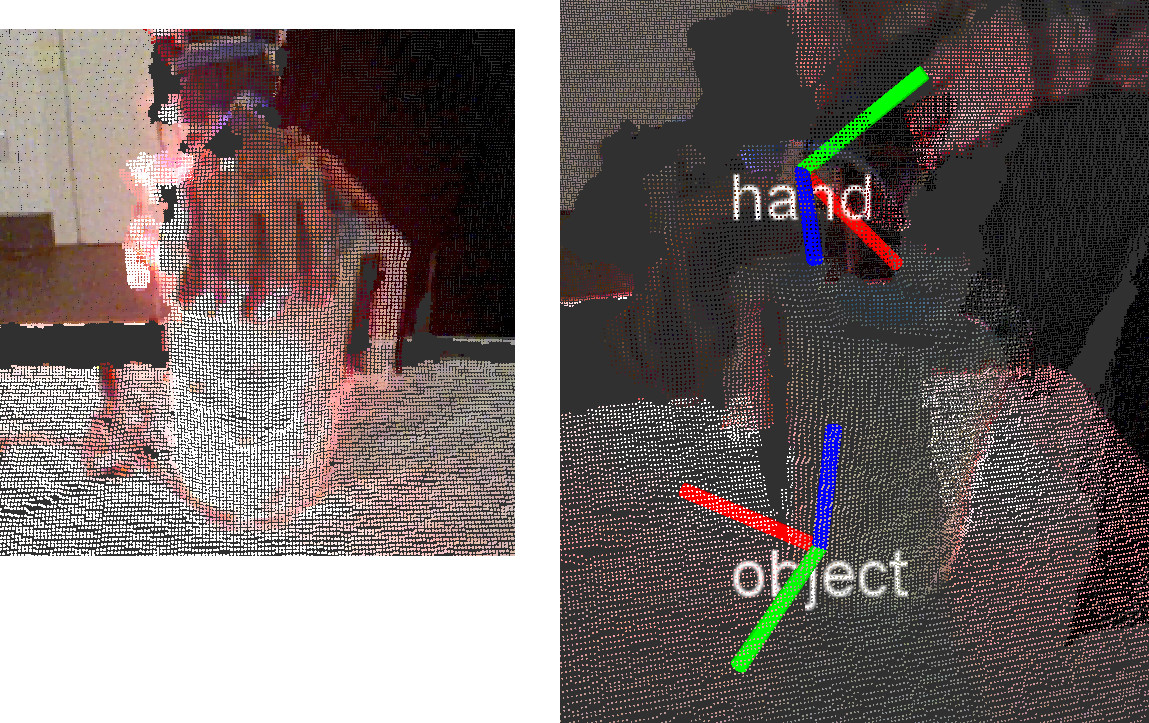
\includegraphics[width=0.95\textwidth]{GRP_data1}
  \caption{Some data extracted from a recording. A point cloud acquired during the grasp phase (left) and another point cloud taken during pre grasp with hand and object pose visible on screen (right).}
  \label{fig:grasp:data1}
\end{figure}
in the software infrastructure during the grasp, a timestamp is also included to give all data a proper timeline. So from the software infrastructure point of view, playing back the recorded bag file is like performing the
same grasp again. Putting things in another way, the user has access to all the information he would have if he had performed the grasp live. In particular the user can extract the following from the bag file:
\begin{figure}[tb!]
  \centering
  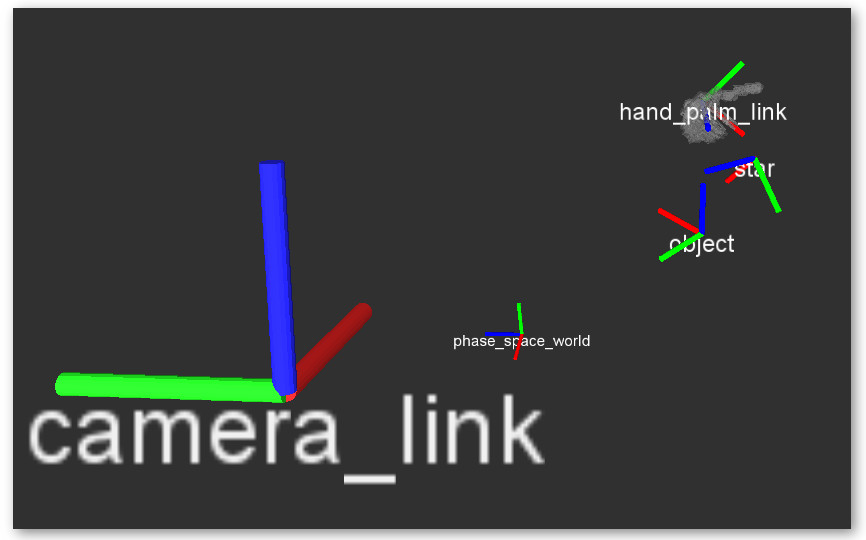
\includegraphics[width=0.95\textwidth]{GRP_data2}
  \caption{Some other data extracted from a recording. The pose of some systems during a grasp are visible on screen, they are from left to right: the Asus camera, the PhaseSpace, the object, the SoftHand palm and the star fixed on the object.}
  \label{fig:grasp:data2}
\end{figure}
\begin{itemize}
  \item Transformations at any given time between all reference systems present: the SoftHand (palm, fingers, phalanges), object, stars, cameras and PhaseSpace.
  \item Readings of finger bending from the FlexiForce glove at any given time.
  \item Point Clouds and images recorded from the camera.
\end{itemize}

This type of approach was preferred, because it's compact and yet leaves the user with the flexibility to chose what to extract, furthermore is easily expandable with additional hardware or improvable for future situations.
Figures.~\ref{fig:grasp:data1} and~\ref{fig:grasp:data2} give some examples of what can be extracted from the recordings.

The dataset is accessible from the project website~\cite{website:pacman:dataset} under ``grasp datasets'' voice. At present day the dataset is still considered to be under development, but it is planned to be improved in number 
and quality of grasps, shortly.
